% arara: pdflatex
% !arara: biber
% !arara: pdflatex
% How to run: 
% 1) pdflatex "filename".tex
% 2) biber "filename"
% 3) pdflatex "filename".tex
% 4) pdflatex "filename".tex


\documentclass[x11names]{article}
\usepackage{verbatim}
\usepackage{listings}
\usepackage{graphicx}
\usepackage{a4wide}
\usepackage{color}
\usepackage{amsmath}
\usepackage{amssymb}
\usepackage[dvips]{epsfig}
\usepackage[T1]{fontenc}
% \usepackage{cite} % [2,3,4] --> [2--4]
\usepackage{shadow}
\usepackage{hyperref}
\usepackage{physics}
\usepackage{url}
\usepackage{tikz}
\usepackage{subcaption}
\usepackage[utf8]{inputenc}
\usepackage{booktabs} % Allows the use of \toprule, \midrule and \bottomrule in tables
\usepackage[font={small,it}]{caption}
\usepackage[margin=0.7in]{geometry} %Sets the margins in the document
\usepackage{siunitx}    %Allows use of SI units macros

%Defines calculator way to write powers of ten
\sisetup{output-exponent-marker=\textsc{e}}


% Change numbering and some commands
\renewcommand\thesection{Exercise \Roman{section}}
\renewcommand\thesubsection{\Roman{section}.\alph{subsection}}

%% references
\usepackage[style=authoryear,
            bibstyle=authoryear,
            backend=biber,
            % refsection=chapter,
            maxbibnames=99,
            maxnames=2,
            firstinits=true,
            uniquename=init,
            natbib=true,
            dashed=false]{biblatex}

\addbibresource{bibliography.bib}
% \addbibresource{top.bib}

% \bibliography{bibliography}
% \bibliography{top}


\usepackage[capitalize]{cleveref}

\setcounter{tocdepth}{2}

\lstset{language=c++}
\lstset{alsolanguage=[90]Fortran}
\lstset{basicstyle=\small}
\lstset{backgroundcolor=\color{white}}
\lstset{frame=single}
\lstset{stringstyle=\ttfamily}
\lstset{keywordstyle=\color{red}\bfseries}
\lstset{commentstyle=\itshape\color{blue}}
\lstset{showspaces=false}
\lstset{showstringspaces=false}
\lstset{showtabs=false}
\lstset{breaklines}


%Used to make nice looking python scripts
\definecolor{keywords}{RGB}{255,0,90}
\definecolor{comments}{RGB}{0,0,113}
\definecolor{red}{RGB}{160,0,0}
\definecolor{green}{RGB}{0,150,0}
 
\lstset{language=Python, 
        basicstyle=\ttfamily\small, 
        keywordstyle=\color{keywords},
        commentstyle=\color{comments},
        stringstyle=\color{red},
        showstringspaces=false,
        identifierstyle=\color{green}}





\title{ Exercise 1 \\ Sommerjobb Numeriske Plasmaoppgaver }
\author{Gullik Vetvik Killie
		}


%%%%%%%%%%%%%%%%%%%%%%%%%%%%%%%%%%%%%%%%%%%%%%%%%%%%%%%%%%%%%%%%%%%%%%%%%%%%%%%%%%%%
% Actual text starts here
%%%%%%%%%%%%%%%%%%%%%%%%%%%%%%%%%%%%%%%%%%%%%%%%%%%%%%%%%%%%%%%%%%%%%%%%%%%%%%%%%%%%
\begin{document}


\maketitle


\section{}

\subsection{}
      \begin{align}
            m\pdv{\vb{v}(t)}{t} &= q \left( \vb{E} +   \vb{v}\cross \vb{B_0} \right); \qquad{} \vb{E} = \vb{0} \qquad{} \text{and} \qquad{} \vb{B_0} = (0,0,B_0)
      \end{align}
      By applying Euler's method on the equation of motion, above, with a static magnetic field  and no electric field we arrive at the following equations for a causal relationship between the next timestep of the positions and velocities dependent on the last timestep.

      \begin{align}
            v_x(t+ h) &= v_x(t) + h \left( \frac{q}{m} v_y(t) B_0 \right)
            \\
            v_y(t+ h) &= v_y(t) - h \left( \frac{q}{m} v_x(t) B_0 \right)
            \\
            x(t + h) &= x(t) + hv_x(t)
            \\
            y(t + h) &= y(t) + hv_y(t)
      \end{align}

      To solve this problem we went through the following fairly straight forward algorithm.

      \begin{enumerate}
            \item Declare variables $h$, $q$, $m$, \(B_0\) and vectors \(v_x\), $v_y$, $x$, and $y$.
            \item Set initial conditions
            \item For loop until counter \(=>\) timesteps. Update \(v_x(t+ h)\), $v_y(t+ h)$, $x(t + h)$ and $y(t + h)$.
            \item Plot and analyze results
      \end{enumerate}


\subsection{Results}
      \subsubsection{Gyration plots}
            \begin{figure}
                  \begin{subfigure}[b]{0.45\textwidth}
                        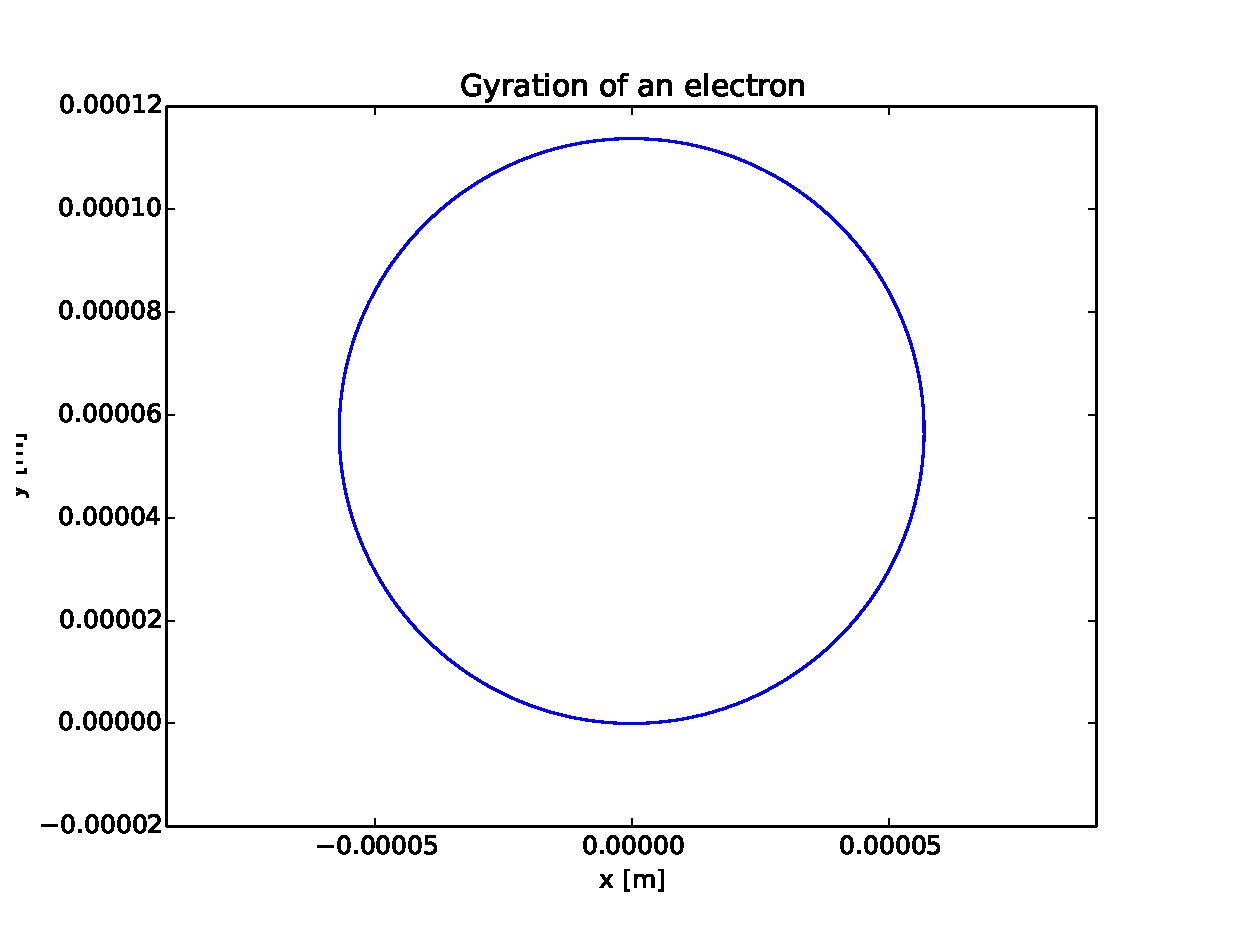
\includegraphics[width = \textwidth]{../source/electronGyration}
                        \caption{Gyration of an electron gyrating in an anti-clockwise direction}
                  \end{subfigure}
                  \begin{subfigure}[b]{0.45\textwidth}
                        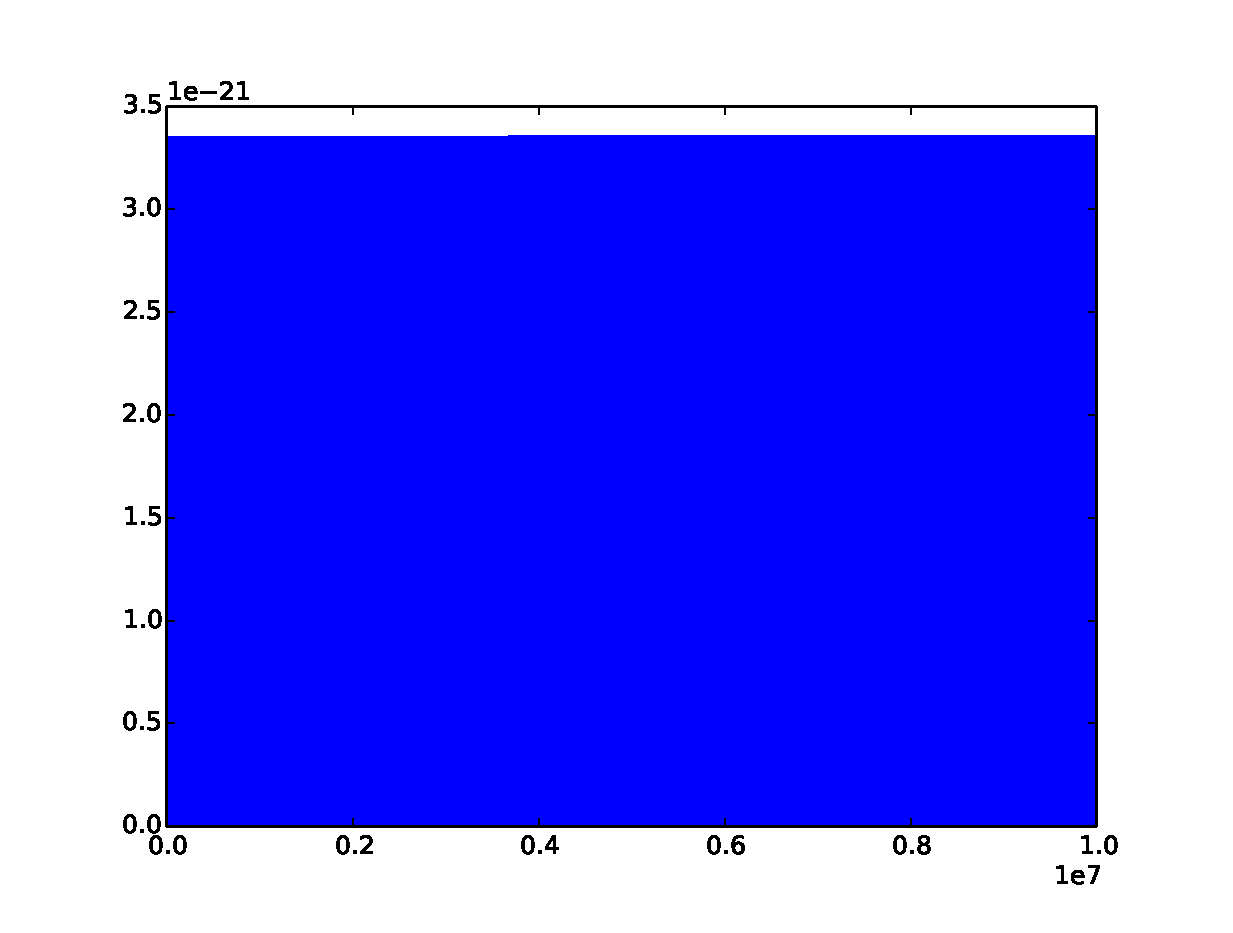
\includegraphics[width = \linewidth]{../source/ionGyration}
                        \caption{Gyration of an oxygen ion gyrating in a clockwise direction}
                  \end{subfigure}
            \end{figure}

      \subsubsection{Gyration radius and frequency}
            From theoretical considerations we can easily calculate the gyration radius, \(\rho\), and gyration frequency, \( \omega_c \), by the following relations, which is valid for a static magnetic field

            \begin{align}
                  \omega_c    &= \frac{qB}{m} \\
                  \rho_c      &= \frac{v_\perp}{\omega_c} = \frac{mv_\perp}{qB}
            \end{align}

            The electron has a mass of \(m = 9.109 \times 10^{-31} \si{kg}\) and a charge of q \( = 1.602\times 10^{-19} \si{\coulomb} \), which is moving in the magnetic field with strength B\(_0\) \( = 5.000 \times 10^ {-5} \si{\tesla}\) and the oxygen ion,  O\(^{+}\), has \(m = 16 \times 1.674 \times 10^{-27} \si{kg}\) and a charge of q \( = 1.602\times 10^{-19} \si{\coulomb} \). The calculated and measured gyration frequencies and radii is written in \cref{tab:results}.




            \begin{table}
                  \centering
                  \begin{tabular}{| c |c | c |}
                        \hline
                                                & e   & O$^+$
                        \\ \hline
                        Theoretical $\rho_c$    &  $5.686 \times 10^{-05} \si{\meter}$   &    $1.672  \si{\meter}$ 
                        \\ \hline
                        Measured $\rho_c$       &  $5.687 \times 10^{-05} \si{\meter}$  &     $1.672 \si{\meter}$ 
                        \\ \hline
                        Theoretical \(\omega_c\)&  $8.794 \times 10^{6} \si{ \radian\per\second} $  & $ 2.991 \times 10 ^{2}\si{ \radian\per\second} $
                        \\ \hline
                        Measured \(\omega_c\)   &  $ 8.793\times 10^{6} \si{ \radian\per\second}$  &  $ 2.991 \times 10 ^{2} \si{ \radian\per\second}$
                        \\ \hline
                  \end{tabular}
                  \caption{The gyration radii and frequencies for an electron and an oxygen ion. For the electron a timestep of \( 10^{-16} \si{s} \) and \(10^7\) steps were used in the simulation, while for the oxygen ion \( 5\times 10^{-8} \si{\second } \) long timesteps and \(10^7\) steps were used. The kinetic energy for the runs had a standard deviation of less than \(\order{10^{-25}}\)}
                  \label{tab:results}
            \end{table}

            

\subsection{Comments regarding the exercise}
      Here I will just list some things that could be helpful to include or things I found unclear.

      \begin{itemize}
            \item It would be nice to specify which oxygen ion is meant (I assumed it was O\(^{2-}\)), but it should affect much results anyway
            \item Change the wording regarding conservation of kinetic energy to mostly conserved, since it doesn't conserve perfectly using an Euler method due to overestimation. The timesteps it started to have good kinetic energy conservation at was \(10^{-16}\) and \( 10^{-9} \) for the electron and ion respectively if you want to include it.
            \item Overflow problems can occur when the timesteps is to big due to the \(  h\frac{qB_0}{m}  \) getting to big. An alternative could be to rewrite the equation of motion to be a unitless equation 
            \( \vb{R} = \frac{\vb{r}-\vb{r}_c}{|\rho_c|}... \), but that adds a complication and makes order of scale intuition abit harder to understand.
            \item Maybe it would be good to remind the students that the gyration frequency is per radian and not per rotation. That could probably reduce some confusion.
            \item The exercise took about $6-7$ hours including writing a report as well.
      \end{itemize}

\appendix
\section{Code}
      

      \lstinputlisting{../source/Single_Particle_Motion.py}


\end{document}